\documentclass[11pt]{article}
\usepackage[utf8]{inputenc}
\usepackage[russian]{babel}
\usepackage{amssymb}
\usepackage{amsmath}
\usepackage{graphicx}
\usepackage{subcaption}
\usepackage{tikz}
\usepackage{array, multirow}
\usetikzlibrary{matrix,calc}
\graphicspath{ {./images/} }

\let\oldemptyset\emptyset
\let\emptyset\varnothing

%isolated term
%#1 - Optional. Space between node and grouping line. Default=0
%#2 - node
%#3 - filling color
\newcommand{\implicantsol}[3][0]{
    \draw[rounded corners=3pt, fill=#3, opacity=0.3] ($(#2.north west)+(135:#1)$) rectangle ($(#2.south east)+(-45:#1)$);
    }


%internal group
%#1 - Optional. Space between node and grouping line. Default=0
%#2 - top left node
%#3 - bottom right node
%#4 - filling color
\newcommand{\implicant}[4][0]{
    \draw[rounded corners=3pt, fill=#4, opacity=0.3] ($(#2.north west)+(135:#1)$) rectangle ($(#3.south east)+(-45:#1)$);
    }

%group lateral borders
%#1 - Optional. Space between node and grouping line. Default=0
%#2 - top left node
%#3 - bottom right node
%#4 - filling color
\newcommand{\implicantcostats}[4][0]{
    \draw[rounded corners=3pt, fill=#4, opacity=0.3] ($(rf.east |- #2.north)+(90:#1)$)-| ($(#2.east)+(0:#1)$) |- ($(rf.east |- #3.south)+(-90:#1)$);
    \draw[rounded corners=3pt, fill=#4, opacity=0.3] ($(cf.west |- #2.north)+(90:#1)$) -| ($(#3.west)+(180:#1)$) |- ($(cf.west |- #3.south)+(-90:#1)$);
}

%group top-bottom borders
%#1 - Optional. Space between node and grouping line. Default=0
%#2 - top left node
%#3 - bottom right node
%#4 - filling color
\newcommand{\implicantdaltbaix}[4][0]{
    \draw[rounded corners=3pt, fill=#4, opacity=0.3] ($(cf.south -| #2.west)+(180:#1)$) |- ($(#2.south)+(-90:#1)$) -| ($(cf.south -| #3.east)+(0:#1)$);
    \draw[rounded corners=3pt, fill=#4, opacity=0.3] ($(rf.north -| #2.west)+(180:#1)$) |- ($(#3.north)+(90:#1)$) -| ($(rf.north -| #3.east)+(0:#1)$);
}

%group corners
%#1 - Optional. Space between node and grouping line. Default=0
%#2 - filling color
\newcommand{\implicantcantons}[2][0]{
    \draw[rounded corners=3pt, opacity=.3] ($(rf.east |- 0.south)+(-90:#1)$) -| ($(0.east |- cf.south)+(0:#1)$);
    \draw[rounded corners=3pt, opacity=.3] ($(rf.east |- 8.north)+(90:#1)$) -| ($(8.east |- rf.north)+(0:#1)$);
    \draw[rounded corners=3pt, opacity=.3] ($(cf.west |- 2.south)+(-90:#1)$) -| ($(2.west |- cf.south)+(180:#1)$);
    \draw[rounded corners=3pt, opacity=.3] ($(cf.west |- 10.north)+(90:#1)$) -| ($(10.west |- rf.north)+(180:#1)$);
    \fill[rounded corners=3pt, fill=#2, opacity=.3] ($(rf.east |- 0.south)+(-90:#1)$) -|  ($(0.east |- cf.south)+(0:#1)$) [sharp corners] ($(rf.east |- 0.south)+(-90:#1)$) |-  ($(0.east |- cf.south)+(0:#1)$) ;
    \fill[rounded corners=3pt, fill=#2, opacity=.3] ($(rf.east |- 8.north)+(90:#1)$) -| ($(8.east |- rf.north)+(0:#1)$) [sharp corners] ($(rf.east |- 8.north)+(90:#1)$) |- ($(8.east |- rf.north)+(0:#1)$) ;
    \fill[rounded corners=3pt, fill=#2, opacity=.3] ($(cf.west |- 2.south)+(-90:#1)$) -| ($(2.west |- cf.south)+(180:#1)$) [sharp corners]($(cf.west |- 2.south)+(-90:#1)$) |- ($(2.west |- cf.south)+(180:#1)$) ;
    \fill[rounded corners=3pt, fill=#2, opacity=.3] ($(cf.west |- 10.north)+(90:#1)$) -| ($(10.west |- rf.north)+(180:#1)$) [sharp corners] ($(cf.west |- 10.north)+(90:#1)$) |- ($(10.west |- rf.north)+(180:#1)$) ;
}

%Empty Karnaugh map 4x4
\newenvironment{Karnaugh}%
{
\begin{tikzpicture}[baseline=(current bounding box.north),scale=0.8]
\draw (0,0) grid (4,4);
\draw (0,4) -- node [pos=0.7,above right,anchor=south west] {cd} node [pos=0.7,below left,anchor=north east] {ab} ++(135:1);
%
\matrix (mapa) [matrix of nodes,
        column sep={0.8cm,between origins},
        row sep={0.8cm,between origins},
        every node/.style={minimum size=0.3mm},
        anchor=8.center,
        ampersand replacement=\&] at (0.5,0.5)
{
                       \& |(c00)| 00         \& |(c01)| 01         \& |(c11)| 11         \& |(c10)| 10         \& |(cf)| \phantom{00} \\
|(r00)| 00             \& |(0)|  \phantom{0} \& |(1)|  \phantom{0} \& |(3)|  \phantom{0} \& |(2)|  \phantom{0} \&                     \\
|(r01)| 01             \& |(4)|  \phantom{0} \& |(5)|  \phantom{0} \& |(7)|  \phantom{0} \& |(6)|  \phantom{0} \&                     \\
|(r11)| 11             \& |(12)| \phantom{0} \& |(13)| \phantom{0} \& |(15)| \phantom{0} \& |(14)| \phantom{0} \&                     \\
|(r10)| 10             \& |(8)|  \phantom{0} \& |(9)|  \phantom{0} \& |(11)| \phantom{0} \& |(10)| \phantom{0} \&                     \\
|(rf) | \phantom{00}   \&                    \&                    \&                    \&                    \&                     \\
};
}%
{
\end{tikzpicture}
}

%Empty Karnaugh map 2x4
\newenvironment{Karnaughvuit}%
{
\begin{tikzpicture}[baseline=(current bounding box.north),scale=0.8]
\draw (0,0) grid (4,2);
\draw (0,2) -- node [pos=0.7,above right,anchor=south west] {yz} node [pos=0.7,below left,anchor=north east] {x} ++(135:1);
%
\matrix (mapa) [matrix of nodes,
        column sep={0.8cm,between origins},
        row sep={0.8cm,between origins},
        every node/.style={minimum size=0.3mm},
        anchor=4.center,
        ampersand replacement=\&] at (0.5,0.5)
{
                      \& |(c00)| 00         \& |(c01)| 01         \& |(c11)| 11         \& |(c10)| 10         \& |(cf)| \phantom{00} \\
|(r00)| 0             \& |(0)|  \phantom{0} \& |(1)|  \phantom{0} \& |(3)|  \phantom{0} \& |(2)|  \phantom{0} \&                     \\
|(r01)| 1             \& |(4)|  \phantom{0} \& |(5)|  \phantom{0} \& |(7)|  \phantom{0} \& |(6)|  \phantom{0} \&                     \\
|(rf) | \phantom{00}  \&                    \&                    \&                    \&                    \&                     \\
};
}%
{
\end{tikzpicture}
}

%Empty Karnaugh map 2x2
\newenvironment{Karnaughquatre}%
{
\begin{tikzpicture}[baseline=(current bounding box.north),scale=0.8]
\draw (0,0) grid (2,2);
\draw (0,2) -- node [pos=0.7,above right,anchor=south west] {b} node [pos=0.7,below left,anchor=north east] {a} ++(135:1);
%
\matrix (mapa) [matrix of nodes,
        column sep={0.8cm,between origins},
        row sep={0.8cm,between origins},
        every node/.style={minimum size=0.3mm},
        anchor=2.center,
        ampersand replacement=\&] at (0.5,0.5)
{
          \& |(c00)| 0          \& |(c01)| 1  \\
|(r00)| 0 \& |(0)|  \phantom{0} \& |(1)|  \phantom{0} \\
|(r01)| 1 \& |(2)|  \phantom{0} \& |(3)|  \phantom{0} \\
};
}%
{
\end{tikzpicture}
}

%Defines 8 or 16 values (0,1,X)
\newcommand{\contingut}[1]{%
\foreach \x [count=\xi from 0]  in {#1}
     \path (\xi) node {\x};
}

%Places 1 in listed positions
\newcommand{\minterms}[1]{%
    \foreach \x in {#1}
        \path (\x) node {1};
}

%Places 0 in listed positions
\newcommand{\maxterms}[1]{%
    \foreach \x in {#1}
        \path (\x) node {0};
}

%Places X in listed positions
\newcommand{\indeterminats}[1]{%
    \foreach \x in {#1}
        \path (\x) node {X};
}

\begin{document}
%         \begin{center}
%         Вариант 7
%         \end{center}
%
%         \textit{\textbf{Задание 1}}
%
%         \textit{Универсальное множество состоит из 26 строчных букв латинского
% алфавита. Заданы множества A, B, C и D. Вычислить мощность множеств X
% и Y.}
%
% \textit{Даны множества
% $A=\{b,f,g,m,o\}, B=\{b,g,h,l,u\}, C=\{e,f,m\}, D=\{e,g,l,p,q,u,v\}$\\
% Вычислить мощность множеств}
% $$X = (A \setminus C) \cup (B \cap C),
% Y=(A \cap \bar B) \cup (D \setminus C) $$
%
% \underline{Решение:}
%
% 1. Определим элементы множества 
% $X = (A \setminus C) \cup (B \cap C)$.
%
% Для этого найдём сначала разность множеств $A \setminus C$.
% Для этого вычеркнем из множества $A=\{b,f,g,m,o\}$ элементы
% $\{f, m\}$, принадлежащие $C=\{e,f,m\}$. Следовательно,
% $A \setminus C = \{b, g, o\}$.
% Затем найдём пересечение множеств $B \cap C$.
% Множества $B$ и $C$ не имеют общих элементов. Следовательно,
% $B \cap C = \emptyset$.
% Таким образом, объединение $(A \setminus C) \cup (B \cap C)$ состоит из
% трёх элементов $\{b, g, o\}$.
%
% Мощность множества 
% $X = (A \setminus C) \cup (B \cap C)$ равна 3.
%
% 2. Определим элементы множества 
% $Y=(A \cap \bar B) \cup (D \setminus C)$
%
% Найдем дополнение B . Универсальное множество по условию задания
% состоит их 26 букв
% $\{a,b,c,d,e,f,g,h,i,j,k,l,m,n,o,p,q,r,s,t,u,v,w,x,y,z\}$.
% Если отсюда исключить 5 элементов множества $B$, то получим множество
% $B$ из 21 элемента
% $\{a,c,d,e,f,i,j,k,m,n,o,p,q,r,s,t,v,w,x,y,z\}$.
%
% Пересечение множеств $A \cap \bar B$
% состоит из элементов $\{f, m, o\}$, т.е. всех
% элементов множества $A$, которые не принадлежат $\bar B$.
%
% Для нахождения разности множеств $D \setminus C$ вычеркнем из множества
% $D=\{e,g,l,p,q,u,v\}$
% элемент $\{e\}$, принадлежащий
% $C=\{e,f,m\}$. Получим
% $D \setminus C = \{g, l, p, q, u, v\}$. В итоге\\
% $$Y=(A \cap \bar B) \cup (D \setminus C) = \{f,g,l,m,o,p,q,u,v\}$$
% Мощность множества Y равна 9. В данном случае множества $D \setminus C$
% и $A \cap \bar B$ не пересекаются и мощность объединения равна
% сумме мощностей слагаемых
%
% Card Y=3+6
%
% \pagebreak
%
% \textit{\textbf{Задание 2}}
%
% \textit{Задайте множество, указанное на рисунке с использованием
% характеристического свойства множества:}
%
% \begin{center}
% 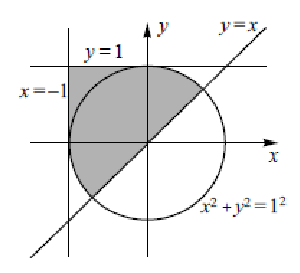
\includegraphics[scale=0.8]{t2}
% \end{center}
%
% \underline{Решение:}
%
% Предлагаем вначале выразить это множество через системы и
% совокупности:
%
% $\left[ 
%   \begin{gathered} 
%     \left\{ 
%       \begin{gathered} 
%                   x^2 + y^2 \leq 1, \hfill 
%         \\ 
%         y \geq x \hfill 
%         \\ 
%       \end{gathered} 
%     \right. \hfill 
%     \\ 
%     \left\{ 
%       \begin{gathered} 
%                   x^2+y^2 \geq 1, \hfill 
%         \\ 
%         y \geq 0, \hfill 
%         \\ 
%         y \leq 1, \hfill 
%         \\ 
%         x \leq 0, \hfill 
%         \\ 
%         x \geq -1, \hfill 
%         \\ 
%       \end{gathered} 
%     \right. \hfill 
%     \\ 
%   \end{gathered} 
% \right.$
% \\[3pt]
%
% Теперь запишем с использованием характеристического
% свойства множества, используя для систем операцию пересечения
% множеств, а для совокупности - объединения:
%
% $$X=\{(x;y) \vert x^2+y^2 \leq 1, y \geq x\} \cup \{(x;y)\vert
% x^2 + y^2 \geq 1, y \geq 0, y \leq 1, x \leq 0, x \geq -1\}$$
%
% \pagebreak
%
% \textit{\textbf{Задание 3}}
%
% Проиллюстрировать равенство при помощи диаграмм Эйлера-Венна:
% $$(A \setminus B) \cup (A \cap C) = A \setminus (B \setminus C)$$
%
% \underline{Решение:}
%
% Построим последовательно левую часть равенства:
%
% \begin{figure}[h]
%         \captionsetup[subfigure]{labelformat=empty}
%         \centering
%         \begin{subfigure}{.32\textwidth}
%                 \centering
%                 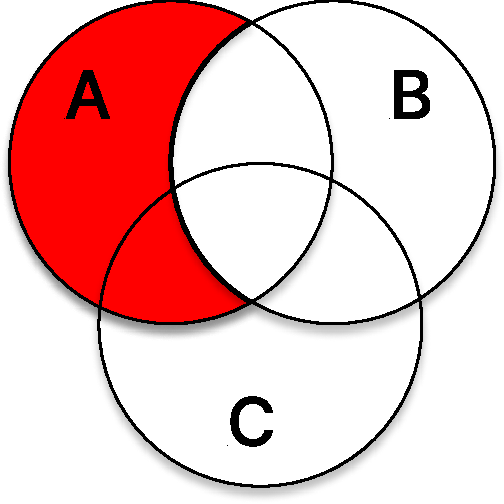
\includegraphics[width=1\linewidth]{t3_1_1.pdf}
%                 \caption{1. $A \setminus B$}
%         \end{subfigure}
%         \begin{subfigure}{.32\textwidth}
%                 \centering
%                 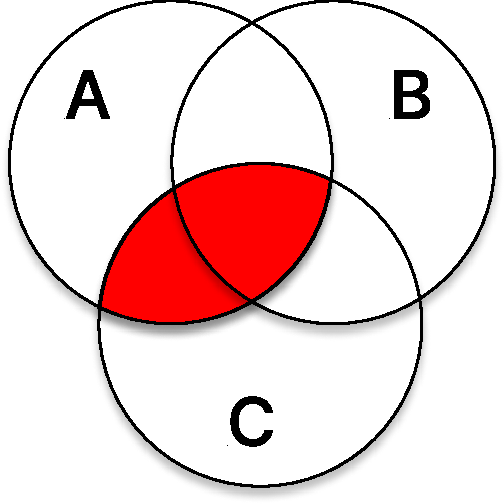
\includegraphics[width=1\linewidth]{t3_1_2.pdf}
%                 \caption{2. $A\cap C$}
%         \end{subfigure}
%         \begin{subfigure}{.33\textwidth}
%                 \centering
%                 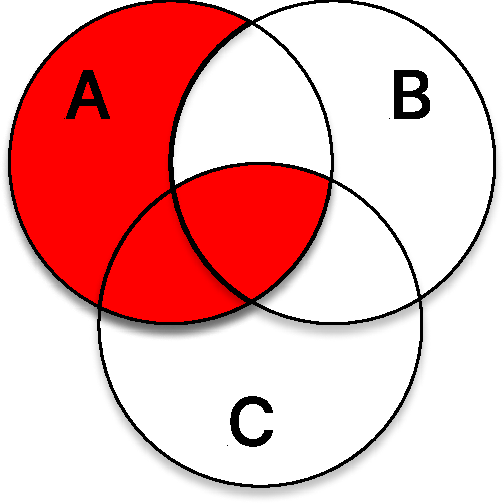
\includegraphics[width=1\linewidth]{t3_1_3.pdf}
%                 \caption{3. $(A \setminus B) \cup (A \cap C)$}
%         \end{subfigure}
% \end{figure}
%
% Теперь построим правую часть:
%
% \begin{figure}[h]
%         \captionsetup[subfigure]{labelformat=empty}
%         \centering
%         \begin{subfigure}{.32\textwidth}
%                 \centering
%                 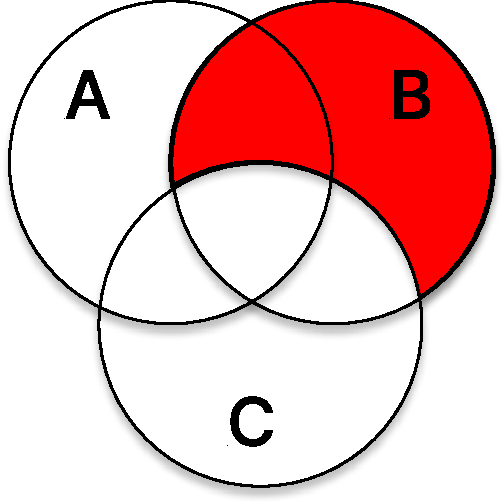
\includegraphics[width=1\linewidth]{t3_2_1.pdf}
%                 \caption{1. $(B \setminus C)$}
%         \end{subfigure}
%         \begin{subfigure}{.32\textwidth}
%                 \centering
%                 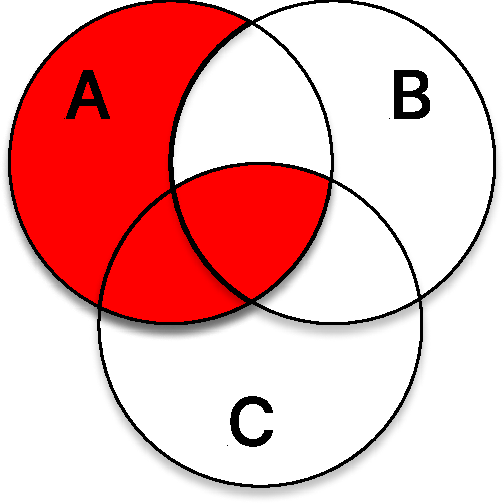
\includegraphics[width=1\linewidth]{t3_2_2.pdf}
%                 \caption{2. $A \setminus (B \setminus C)$}
%         \end{subfigure}
% \end{figure}
%
% Диаграммы для левой и правой части оказались одинаковы!

% \pagebreak
%
% \textit{\textbf{Задание 4.}}
%
% \textit{Отношение задано матрицей. Исследовать отношение на симметрию,
% антисимметрию, асимметрию, рефлексивность, антирефлексивность. Найти
% транзитивное замыкание отношения.}
%
% $$M=
% \begin{pmatrix}
%         0 & 0 & 0 & 1\\
%         0 & 1 & 1 & 0\\
%         0 & 0 & 1 & 1\\
%         0 & 0 & 0 & 1
% \end{pmatrix}.$$
%
% \underline{Решение:}
%
% 1. Данное отношение не является симметричным, так как матрица
% несимметрична. Например, пара (2,3) принадлежит данному отношению, а пара
% (3,2) ему не принадлежит.
%
% 2. Отношение антисимметрично, так как нет ни одной пары\\
% $m_{ij} = m_{ji} = 1, i \neq j$.
%
% 3. Отношение антисимметрично, но не асимметрично, так как на
% диагонали матрицы имеются элементы равные 1.
%
% 4. Не все диагональные элементы метрицы равняются 1.
% Данное отношение не является рефлексивным
%
% 5. Отношение не обладает свойством антирефлексивности, так как
% не все диагональные элементы являются нулевыми
%
% Найдем транзитивное замыкание данного отношения по алгоритму
% Уоршолла:
%
% Рассматриваем все внедиагональные $(i \neq j)$ элементы матрицы.
% Если $m_{ij}=1$, то $i$-ю строку заменяем дизъюнкцией $i$-й и $j$-й строк.
%
% 1. Элемент $m_{14}=1$. Первую строку заменяем поэлементной
% дизъюнкцией первой и четвертой строки:
%
% $$M_1=
% \begin{pmatrix}
%         0 & 0 & 0 & 1\\
%         0 & 1 & 1 & 0\\
%         0 & 0 & 1 & 1\\
%         0 & 0 & 0 & 1
% \end{pmatrix}.$$
%
% Данное отношение не является транзитивным, так как, например, пары
% (1,2) и (2,4) не принадлежат данному отношению, а пара (1,4)
% ему принадлежит.
%
% 2. Элемент $m_{23} = 1$. Вторую строку заменяем поэлементной
% дизъюнкцией второй и третьей строки:
%
% $$M_2=
% \begin{pmatrix}
%         0 & 0 & 0 & 1\\
%         0 & 1 & 1 & 1\\
%         0 & 0 & 1 & 1\\
%         0 & 0 & 0 & 1
% \end{pmatrix}.$$
%
% 3. Элемент $m_{34} = 1}. Дизъюнкция третьей и четвертой строки не меняет
% вид матрицы. Таким образом, полученная матрица $M_2$ является матрицей
% транзитивного замыкания нашего отношения
% \\[10pt]
%
% \textit{\textbf{Задание 5.}}
%
% На множестве упорядоченных пар $x_0=(0,0), x_1=(1,0), x_2=(0,1),\\
% x_3=(1,1)$ задана бинарная мультипликативная операция. Произведение задано
% по правилу $A*B=(a_2b_2, a_1b_2)$. Является ли полугруппой структура
%  $(X,*)$, где $X=\{x_0, x_1, x_2, x_3\}$? Составить таблицу Кэли структуры.
%
%  \underline{Решение:}
%
% Проверим ассоциативность введенного произведения — необходимое
% свойство для того, чтобы алгебраическая структура была полугруппой.
% Рассмотрим произведение $A*(B*C)$ трёх произвольных пар из X:
%
% $$A=(a_1, a_2), B=(b_1, b_2), C=(c_1, c_2).$$
%
% Найдём сначала произведение $B*C=(b_2c_2, b_1c_2)$, затем получим
% $A*(B*C)=(a_2b_1c_2, a_1b_1c_2).$
%
% Аналогично:
%
% $$(A*B)*C=(a_2b_2,a_1b_2)*(c_1,c_2)=(a_1b_2c_2,a_2b_2c_2)$$
%
% Очевидно, $A*(B*C) \neq (A*B)*C$, т.е. операция умножения не ассоциативна
% и алгебраическая структура $(X, *)$ не является полугруппой. Составим таблицу Кэли.
%
% \begin{center}
%         \begin{tabular}{ |c|c|c|c|c| }
%                 \hline
%                 $*$ & $x_0$ & $x_1$ & $x_2$ & $x_3$\\
%                 \hline
%                 $x_0$ & $x_0$ & $x_0$ & $x_0$ & $x_0$\\
%                 \hline
%                 $x_1$ & $x_0$ & $x_0$ & $x_2$ & $x_2$\\
%                 \hline
%                 $x_2$ & $x_0$ & $x_0$ & $x_1$ & $x_1$\\
%                 \hline
%                 $x_3$ & $x_0$ & $x_0$ & $x_3$ & $x_3$\\
%                 \hline
%         \end{tabular}
% \end{center}
%
% \pagebreak
%
% \textit{\textbf{Задание 6:}}
%
% Построив соответствующую таблицу значений, выясните, равны ли
% следующие булевы функции
%
% $$f(x,y,z)=xy' \lor x'y \lor x'z',
% \ g(x,y,z)=(x' \lor y')(x \lor y \lor z')$$
%
% \underline{Решение:}
%
% Построим таблицы значений для функций $f$ и $g$:
%
% $$f(x,y,z)=x y' \lor x' y \lor x'z'$$
%
% \begin{center}
%         \begin{tabular}{ |c|c|c|c|c|c|c|c|c|c|c| }
%                 \hline
%                 $x$ & $y$ & $z$ & $x'$ & $y'$ & $z'$ & $xy'$ & $x'y$ & $x' z'$ & $f(x,y,z)$\\
%                 \hline
%                 0 & 0 & 0 & 1 & 1 & 1 & 0 & 0 & 1 & 1\\
%                 \hline
%                 0 & 0 & 1 & 1 & 1 & 0 & 0 & 0 & 0 & 0\\
%                 \hline
%                 0 & 1 & 0 & 1 & 0 & 1 & 0 & 1 & 1 & 1\\
%                 \hline
%                 0 & 1 & 1 & 1 & 0 & 0 & 0 & 1 & 0 & 1\\
%                 \hline
%                 1 & 0 & 0 & 0 & 1 & 1 & 1 & 0 & 0 & 1\\
%                 \hline
%                 1 & 0 & 1 & 0 & 1 & 0 & 1 & 0 & 0 & 1\\
%                 \hline
%                 1 & 1 & 0 & 0 & 0 & 1 & 0 & 0 & 0 & 0\\
%                 \hline
%                 1 & 1 & 1 & 0 & 0 & 0 & 0 & 0 & 0 & 0\\
%                 \hline
%         \end{tabular}
% \end{center}
%
% $$g(x,y,z)=(x' \lor y')(x \lor y \lor z')$$
%
% \begin{center}
%         \begin{tabular}{ |c|c|c|c|c|c|c|c|c| }
%                 \hline
%                 $x$ & $y$ & $z$ & $x'$ & $y'$ & $z'$ & $x' \lor y'$ & $x \lor y \lor z'$ & $g(x,y,z)$\\
%                 \hline
%                 0 & 0 & 0 & 1 & 1 & 1 & 1 & 1 & 1\\
%                 \hline
%                 0 & 0 & 1 & 1 & 1 & 0 & 1 & 0 & 0\\
%                 \hline
%                 0 & 1 & 0 & 1 & 0 & 1 & 1 & 1 & 1\\
%                 \hline
%                 0 & 1 & 1 & 1 & 0 & 0 & 1 & 1 & 1\\
%                 \hline
%                 1 & 0 & 0 & 0 & 1 & 1 & 1 & 1 & 1\\
%                 \hline
%                 1 & 0 & 1 & 0 & 1 & 0 & 1 & 1 & 1\\
%                 \hline
%                 1 & 1 & 0 & 0 & 0 & 1 & 0 & 1 & 0\\
%                 \hline
%                 1 & 1 & 1 & 0 & 0 & 0 & 0 & 1 & 0\\
%                 \hline
%         \end{tabular}
% \end{center}
%
% Получили:\\
% $$f(x,y,z)=g(x,y,z)$$
%
% \pagebreak

% \textit{\textbf{Задание 7:}}
%
% \textit{Постройте минимальную ДНФ для функции тремя разными
% способами (графическим способом, картами Карно, методом Квайна):}\\
% $f=10111010$
%
% \underline{Решение:}
%
% В данной функции восемь бит, т.е. это функция трех переменных. Будем
% считать этими переменными $x$, $y$ и $z$.
% В данной функции нулей меньше, поэтому быстрее через них. Разряды:
%
% $$\overset{0}{1} \overset{1}{0} \overset{2}{1} \overset{3}{1} \overset{4}{1} \overset{5}{0} \overset{6}{1} \overset{7}{0}$
%
% тогда нулям соответствуют наборы переменных 001, 101 и 111, а все остальные
% наборы – это единицы.
%
% Минимизация графическим способом (метод гиперкубов)
%
% Нарисуем единичный куб в системе координат и выделим его вершины,
% координаты которых соответствуют наборам переменных, на которых наша
% функция принимает значения 1, и выколем те вершины, которые соответствуют
% наборам, на которых принимается значение 0.
%
% 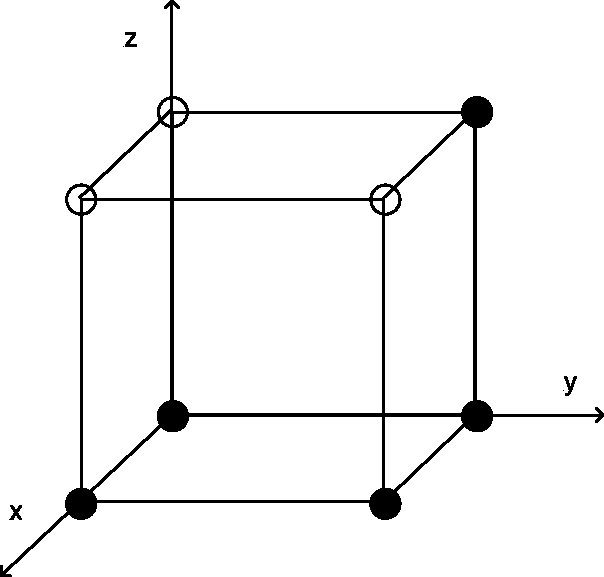
\includegraphics{t7.pdf}
%
% Теперь пробуем покрыть выделенные точки, не зацепив невыделенные
% минимальным количеством сначала граней (у нас это не возможно), затем ребер
% (у нас все точки покрываются минимально тремя ребрами (выделены на
% рисунке ниже), затем, если не удалось ничем ранее, отдельными вершинами.
%
% 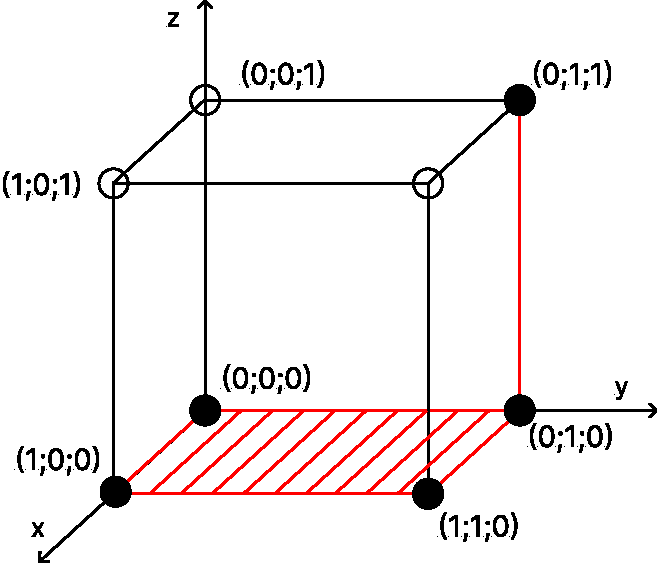
\includegraphics{t7_2.pdf}
%
% Для каждого из выделенных объектов (граней, ребер или вершин)
% посмотрим, какие переменные (координаты) не менялись. Для этих переменных
% составим конъюнктивные одночлены по правилу построения СДНФ. Например,
% для грани, соединяющей точки с координатами $(1;0;0),\\ (0;0;0), (0;1;0), (1;1;0)$
% не меняются третья координата (соответствует z), и онa
% равнa нулю, значит соответствующий конъюнктивный одночлен $z'$, а для
% ребра, соединяющего точки (0;1;0) и (0;1;1) не меняются первая и вторая координаты (x и y соответственно), причем x=0, а y=1, тогда получим одночлен $x'y$.
%
% Ответ: $f=z' \lor x'y$
%
% \textit{Минимизация методом карт Карно}
%
% Составим двумерную таблицу значений нашей функции разделив
% переменные произвольным образом на две группы (предлагаем разделить на $x$ и
% $yz$ просто из-за того, что такая запись будет более протяженной горизонтально).
% Сочетания переменных упорядочим по коду Грея. Кодом Грея называется
% двоичный код, у которого два соседних значения различаются не более чем в
% одной позиции. Получим:
%
% \begin{center}
% \begin{Karnaughvuit}
%        \minterms{0,2,3,4,6}
%         \maxterms{1,5,7}
% \end{Karnaughvuit}
% \end{center}
%
% С помощью прямоугольников площадью кратной степени 2, покрываем
% все единицы, не задевая нули. При этом ячейки, которые находятся на
% противоположных концах (как по горизонтали, так и по вертикали, но не по
% диагонали) считаются смежными. Прямоугольники могут пересекаться.
%
% У нас получится:
%
% \begin{center}
% \begin{Karnaughvuit}
%        \minterms{0,2,3,4,6}
%         \maxterms{1,5,7}
%     \implicantcostats{0}{6}{green}
%        \implicant{3}{2}{red}
% \end{Karnaughvuit}
% \end{center}
%
% Каждый из прямоугольников описывается в виде конъюнктивного
% одночлена, как и для графического способа. Получим:
%
% $$f=z' \lor x'y$$
%
% \textit{Минимизация методом Квайна}
%
% Выписываем все совершенные одночлены, для которых $f=1$. Во втором
% столбце для удобства проведем их группировку по числу нулей в их записи.
%  % 10111010
% \begin{center}
% \begin{tabular}{|c|c|}\hline
%     000 & 000\\
%     \cline{2-2}
%     010 & 010\\
%     011 & 100\\
%     \cline{2-2}
%     100 & 011\\
%     110 & 110\\
%     \hline
% \end{tabular}
% \end{center}
%
% Если в одночленах получается разница ровно в одной позиции, то
% заменяем «-».
%
% В этом плане группировка удобна тем, что можно проверять только
% одночлены из соседних групп, например, первый из первой группы и первый из
% второй, первый из первой группы и второй из второй и т.д.
%
% Помечаем одночлены, которые в этом участвовали. Результаты поместим
% в третий столбец. Получим:
%
% \begin{center}
% \begin{tabular}{|c|c|c|}\hline
%     000 & *000 & 0-0\\
%     \cline{2-2}
%     010 & *010 & -00\\
%     011 & *100 & 01-\\
%     \cline{2-2}
%     100 & *011 & -10\\
%     110 & *110 & 1-0\\
%     \hline
% \end{tabular}
% \end{center}
%
% Для удобства сгруппируем теперь по местоположению «прочерка»:
%
% \begin{center}
% \begin{tabular}{|c|c|c|c|}\hline
%     000 & *000 & 0-0 & -00\\
%     \cline{2-2}
%     010 & *010 & -00 & -10\\
%     \cline{4-4}
%     011 & *100 & 01- & 0-0\\
%     \cline{2-2}
%     100 & *011 & -10 & 1-0\\
%     \cline{4-4}
%     110 & *110 & 1-0 & 01-\\
%     \hline
% \end{tabular}
% \end{center}
%
% Продолжаем этот процесс (объединения) пока возможно, считая прочерк
% третьим символом. При этом, с учетом последнего разбиения на группы, мы
% можем работать только в одной группе (нельзя объединить элементы разных
% групп). Не забывайте ставить пометки тех элементов, которые вы объединяете.
% Это важно!
%
% \begin{center}
% \begin{tabular}{|c|c|c|c|c|}\hline
% 	000 & *000 & 0-0 & *-00 & --0\\
%     \cline{2-2}
% 	010 & *010 & -00 & *-10 &\\
%     \cline{4-4}
% 	011 & *100 & 01- & *0-0 &\\
%     \cline{2-2}
% 	100 & *011 & -10 & *1-0 &\\
%     \cline{4-4}
% 	110 & *110 & 1-0 & 01- &\\
%     \hline
% \end{tabular}
% \end{center}
%
% \begin{center}
% \begin{tabular}{|c|c|c|}\hline
% 	& 01- & --0\\
% 	\hline
% 	000 & & +\\
% 	\hline
% 	010 & + & +\\
% 	\hline
% 	011 & + & \\
% 	\hline
% 	100 & & +\\
% 	\hline
% 	110 & & +\\
%     \hline
% \end{tabular}
% \end{center}
%
% Отбираем минимальное число столбцов, с суммарным минимальным
% числом переменных так, чтобы они покрыли все строки. Для этого вначале
% определим те одночлены, которые войдут в ядро (в этих строках только один
% «+», поэтому для них альтернативы нет). У нас это первый, третий, четвертый, пятый столбцы,
% значит одночлены 01- и --0 обязательно войдут в ответ. В результате получим,
% что «+», соответствующие выбранным одночленам у нас автоматически будут в
% 1, 2, 3, 4, 5 строка.
%
% $$f=x'y \lor z'$$
%
% \pagebreak

\textit{\textbf{Задание 8.}}

Для функции, заданной в векторном виде постройте полином 
Жегалкина тремя разными способами (методом неопределенных 
коэффициентов, преобразованием СДНФ, с использованием треугольника): 
$f=01110010$.

Сначала необходимо построить таблицу истинности данной булевой
функции $f(x_1,x_2,x_3)$

\begin{center}
        \begin{tabular}{ |c|c|c|c| }
                \hline
				$x$ & $y$ & $z$ & $f(x_1,x_2,x_3)$\\
                \hline
				0 & 0 & 0 & 0\\
                \hline
				0 & 0 & 1 & 1\\
                \hline
				0 & 1 & 0 & 1\\
                \hline
				0 & 1 & 1 & 1\\
                \hline
				1 & 0 & 0 & 0\\
                \hline
				1 & 0 & 1 & 0\\
                \hline
                1 & 1 & 0 & 1\\
                \hline
                1 & 1 & 1 & 0\\
                \hline
        \end{tabular}
\end{center}

Общий вид полинома Жегалкина для функции трех переменных:

$$f(x_1,x_2,x_3)=a_0+a_1x_1+a_2x_2+a_3x_3+a_{12}x_1x_2+a_{13}x_1x_3+a_{23}x_2x_3+a_{123}x_1x_2x_3$$

Последовательно подставляем наборы значений переменных и находим
коэффициенты $a_0,a_1,...,a_{123}$

$f(0,0,0)=a_0=0$

$f(0,0,1)=a_0 + a_3=1 \Rightarrow 0 + a_3 = 1 \Rightarrow a_3 = 1$

$f(0,1,0)=a_0 + a_2=1 \Rightarrow 0 + a_2 = 1 \Rightarrow a_2=1$

$f(0,1,1)=a_0 + a_2 + a_3 + a_{23}=1 \Rightarrow 0 + 1 + 1 + a_{23}=1 \Rightarrow a_{23} = 1$

$f(1,0,0)=a_0 + a_1=0 \Rightarrow 0 + a_1=0 \Rightarrow a_1 = 0$

$f(1,0,1)=a_0 + a_1 + a_3 + a_{13}=0 \Rightarrow 0 + 0 + 1 + a_{13}=0 \Rightarrow a_{13}=1$

$f(1,1,0)=a_0 + a_1 + a_2 + a_{12}=1 \Rightarrow 0 + 0 + a_{12}=1 \Rightarrow a_{12}=0$

$f(1,1,1)=a_0 + a_1 + a_2 + a_3 + a_{12} + a_{13} + a_{23} + a_{123}=0 \Rightarrow 0 + 0 + 1 + 1 + 1 + 1 + 1 + 1 + a_{123} = 0 \Rightarrow a_{123}=0$

Подставляя найденные коэффициенты, получаем полином Жегалкина:

$f(x_1,x_2,x_3)= x_2 + x_3 + x_1x_3 + x_2x_3$

\textbf{Метод треугольника Паскаля}

Построим полином Жегалкина, используя треугольник Паскаля.

\begin{center}
        \begin{tabular}{ |c|c|c|c|c|c| }
                \hline
				$x_1$ & $x_2$ & $x_3$ & $f(x_1,x_2,x_3)$ & Треугольник Паскаля & Слагаемые\\
                \hline
				0 & 0 & 0 & 0 & 0 1 1 1 0 0 1 0 & 1\\
                \hline
				0 & 0 & 1 & 1 &[1] 0 0 1 0 1 1 \ & x_3\\
                \hline
				0 & 1 & 0 & 1 & [1] 0 1 1 1 0 \ & x_2\\
                \hline
				0 & 1 & 1 & 1 & [1] 1 0 0 1 \ & x_2x_3\\
                \hline
				1 & 0 & 0 & 0 & 0 1 0 1 & x_1\\
                \hline
				1 & 0 & 1 & 0 & [1] 1 1 \ & x_1x_3\\
                \hline
				1 & 1 & 0 & 1 & 0 0 & x_1x_2\\
                \hline
				1 & 1 & 1 & 0 & 0 & x_1x_2x_3\\
                \hline
        \end{tabular}
\end{center}

Поясним, как заполняется треугольник Паскаля. Верхняя строка
треугольника задает вектор значений булевой функции $f=(01110010)$.В каждой
строке, начиная со второй, любой элемент такого треугольника вычисляется
как сумма по модулю 2 двух соседних элементов предыдущей строки.

Левой стороне треугольника Паскаля соответствует наборы значений
переменных исходной функции $f(x_1,x_2,x_3)$. Соединяя знаком конъюнкции
переменные значения которых в наборе равны 1, мы получим слагаемое в
полиноме Жегалкина. Набору (000) соответствует 1, набору (001) соответствует $x_3$
и т.д

Полином Жегалкина:

$f(x_1,x_2,x_3)= x_2 + x_3 + x_1x_3 + x_2x_3$

\textbf{Преобразование ДНФ}

По таблице истинности построим СДНФ (метод работает только для
СДНФ, просто для ДНФ так делать нельзя!):

\begin{center}
        \begin{tabular}{ |c|c|c|c| }
                \hline
				$x_1$ & $x_2$ & $x_3$ & $f(x_1,x_2,x_3)$\\
                \hline
				0 & 0 & 0 & 0\\
                \hline
				0 & 0 & 1 & 1\\
                \hline
				0 & 1 & 0 & 1\\
                \hline
				0 & 1 & 1 & 1\\
                \hline
				1 & 0 & 0 & 0\\
                \hline
				1 & 0 & 1 & 0\\
                \hline
                1 & 1 & 0 & 1\\
                \hline
                1 & 1 & 1 & 0\\
                \hline
        \end{tabular}
\end{center}

Для построения СДНФ по таблице истинности выбираем наборы, на
которых функция f принимает значение, равное 1. Если значение переменной в
этом наборе равно 0, то она берется с отрицанием, если значение переменной
равно 1, то переменная берется без отрицание. Соединив знаком конъюнкции
переменные соответствующего набора, получим элементарную конъюнкцию.
Тогда дизъюнкция всех таких элементарных конъюнкций есть СДНФ.

$$f(x_1,x_2,x_3)=\bar x_1 \bar x_2 x_3 \lor \bar x_1 x_2 \bar x_3 \lor \bar x_1 x_2x_3 \lor x_1x_2 \bar x_3.$$

Теперь просто заменим дизьюнкцию суммой Жегалкина (так можно
сделать из-за того, что СДНФ устроена так, что в каждый одночлен входят ВСЕ
переменные, т.е. как минимум одна переменная будет входить в данные
одночлены как с отрицанием, так и без него, т.е. при применении формулы $a \lor b = a + b + ab$, конъюнкция будет равна 0.

$$f(x_1,x_2,x_3)=\bar x_1 \bar x_2 x_3 + \bar x_1 x_2 \bar x_3 + \bar x_1 x_2x_3 + x_1x_2 \bar x_3.$$

Теперь, воспользовавшись свойством $\bar a = a + 1$ и раскрыв скобки
получим:

$f(x_1,x_2,x_3)=\bar x_1 \bar x_2 x_3 + \bar x_1 x_2 \bar x_3 + \bar x_1 x_2x_3 + x_1x_2 \bar x_3 = $

$ = (x_1 + 1)(x_2 + 1)x_3 + (x_1 + 1)x_2(x_3 + 1) + (x_1 + 1)x_2x_3 + x_1x_2(x_3 + 1) = $

$ = (x_1x_2x_3 + x_1x_3 + x_2x_3 + x_3) + (x_1x_2x_3 + x_1x_2 + x_2x_3 + x_2) + $

$ + (x_1x_2x_3 + x_2x_3) + (x_1x_2x_3 + x_1x_2).$

И, наконец, воспользуемся свойством0a a  , т.е. уберем все скобки и
все члены, встречающиеся ЧЕТНОЕ число раз вычеркнем. Получим:

$f(x_1,x_2,x_3)= x_1x_3 + x_2x_3 + x_3 + x_2$

\pagebreak

\textbf{\textit{Задание 9.}}

Для булевой функции найдите представляющий ее полином Жегалкина:

$$x'y'z' \lor x'yz' \lor x'yz \lor xy'z \lor xyz'$$

\textit{Решение:}

Для нахождения полинома Жегалкина нужно выразить все
встречающиеся в данном выражении булевы функции через сумму Жегалкина
(сложение по модулю 2) и конъюнкцию, а затем, пользуясь свойствами
функций, максимально упростить полученное выражение. Проделаем это для
данной булевой функции:

$x'y'z' \lor x'yz' \lor x'yz \lor xy'z \lor xyz' = x'y'z' + x'yz' + x'yz + xy'z + xyz' =$

$= (x+1)(y+1)(z+1) + (x+1)y(z+1)+(x+1)yz+x(y+1)z+xy(z+1)=$

$ = (xy + x + y + 1)(z+1) + (xy + y)(z+1)+(xyz+yz)+(xy+x)z+$

$ + (xyz+xy)=$

$=(xyz + xy + xz + x + yz + y + z + 1) + (xyz + xy + yz + y) + $

$ + (xyz + yz) + (xyz + xz) + (xyz + xy) =$

$ = 1 + x + z + xy + yz + xyz$

\end{document}
